% -*- latex -*-
% c4.tex
% LabSK 13.06.2022

% Wymagane pola (komentarz):
% Dawid Chmielewski				% Imię Nazwisko

\documentclass[a4paper,11pt]{article}

\usepackage[T1]{polski}
\usepackage[utf8]{inputenc}  			% Kodowanie pliku
\usepackage{pdfpages}

\hoffset=-3.0cm                         % Mniejszy lewy margines
\textwidth=18cm                         % szerzej
\evensidemargin=0pt

\voffset=-3cm                           % Mniejszy górny margines
\textheight=27cm                        % szerzej wzdłuż

\setlength{\parindent}{0pt}             % Paragraf od początku linii
\setlength{\parskip}{\medskipamount}    % Odstęp pomiędzy paragrafami
\raggedbottom                           % bez rozciągania strony

% Dodatkowe komendy
\newcommand\BS{\char`\\}                % \BS == back-slash
\newcommand\TY{\raise.17ex\hbox{$\scriptstyle\mathtt{\sim}$}}   % \TY == większa tylda w \tt

\thispagestyle{empty}			        % bez numeracji stron
\usepackage{enumerate}

\begin{document}
\title{ Sieci komputerowe - sprawozdanie z ćwiczenia 7. }
\author{ Dawid Chmielewski, numer indeksu: 311188 }
\date{13 czerwca 2022}

\maketitle{Temat ćwiczenia: sieci publiczne i NAT}

Podczas realizacji ćwiczenia korzystałem z internetu w Domu Studenckim Bratniak Politechniki Warszawskiej.

\section{Mój prywatny adres IP}

Za pomocą strony whatismyip.com odczytałem adres IP- 194.29.137.12.


\section{Trasa do volta}

Trasę do volta zbadałem za pomocą tracert oraz Test-NetConnection.

\begin{verbatim}
PS C:\Users\Dawid> tracert volt.zet.pw.edu.pl

Tracing route to volt.zet.pw.edu.pl [194.29.146.3]
over a maximum of 30 hops:

  1    <1 ms     3 ms     1 ms  10.12.0.1
  2     *        *       <1 ms  10.255.255.40
  3    <1 ms    <1 ms    <1 ms  ci-to-nat.rtr.ds.pw.edu.pl [194.29.137.57]
  4    <1 ms     *       <1 ms  194.29.132.238
  5     2 ms     5 ms     2 ms  volt.iem.pw.edu.pl [194.29.146.3]
  6    <1 ms    <1 ms    <1 ms  volt.iem.pw.edu.pl [194.29.146.3]

Trace complete.
PS C:\Users\Dawid>
\end{verbatim}

Test-NetConnection:

\begin{verbatim}
PS C:\Users\Dawid> Test-NetConnection -TraceRoute volt.zet.pw.edu.pl -Verbose
VERBOSE: volt.zet.pw.edu.pl
VERBOSE: volt.zet.pw.edu.pl
VERBOSE: Perform operation 'Invoke CimMethod' with following parameters, 
''className' = MSFT_NetAddressFilter,'methodName' = QueryIsolationType,'namespaceName' = 
root\standardcimv2'.
VERBOSE: Operation 'Invoke CimMethod' complete.

ComputerName           : volt.zet.pw.edu.pl
RemoteAddress          : 194.29.146.3
InterfaceAlias         : Ethernet
SourceAddress          : 10.12.5.8
PingSucceeded          : True
PingReplyDetails (RTT) : 0 ms
TraceRoute             : 10.12.0.1
                         10.255.255.40
                         194.29.137.57
                         194.29.132.238
                         194.29.146.3
                         194.29.146.3


PS C:\Users\Dawid>
\end{verbatim}

\section{Trasa z volta do maszyny domowej}

Trasownik w Domu Studenckim nie daje możliwości odpowiedzi na traceroute, więc użyłem icmp.

\begin{verbatim}
volt% traceroute -I -a 194.29.137.12
traceroute to 194.29.137.12 (194.29.137.12), 64 hops max, 72 byte packets
 1  [AS12464] gate (194.29.146.1)  1.772 ms  4.792 ms  1.591 ms
 2  [AS12464] ee-coi.rtr.pw.edu.pl (194.29.132.25)  0.269 ms *  0.222 ms
 3  [AS12464] coi-ee.ee.pw.edu.pl (194.29.132.225)  0.397 ms  0.540 ms  0.417 ms
 4  [AS12464] bratniak.nat.ds.pw.edu.pl (194.29.137.12)  0.265 ms  0.280 ms  0.267 ms
volt%
\end{verbatim}

\section{Pomiar czasu 20 pakietów wysłanych na volta}

\begin{verbatim}
Ping statistics for 194.29.146.3:
    Packets: Sent = 20, Received = 20, Lost = 0 (0% loss),
Approximate round trip times in milli-seconds:
    Minimum = 0ms, Maximum = 9ms, Average = 0ms
\end{verbatim}

\section{Maszyna wirtualna}

Połączenie przez ssh z maszyną uzyskałem dzięki właściwej jej konfiguracji w VirtualBox.

\begin{verbatim}
PS C:\Users\Dawid> ssh -p 3022 dawid@127.0.0.1
dawid@127.0.0.1's password:
Welcome to Ubuntu 22.04 LTS (GNU/Linux 5.15.0-33-generic x86_64)
(...)
\end{verbatim}

Maszyna ma dostęp do internetu, co sprawdziłem poleceniem ping.

\begin{verbatim}

dawid@dawid-VirtualBox:~$ ping -c1 onet.pl
PING onet.pl (75.2.92.173) 56(84) bytes of data.
64 bytes from aafc88a28d9997374.awsglobalaccelerator.com (75.2.92.173): icmp_seq=1 ttl=116 time=2.55 ms

--- onet.pl ping statistics ---
1 packets transmitted, 1 received, 0% packet loss, time 0ms
rtt min/avg/max/mdev = 2.547/2.547/2.547/0.000 ms
dawid@dawid-VirtualBox:~$

\end{verbatim}

\section{Trasa ze stacji s1 do maszyny domowej}

\begin{verbatim}

stud@s1 ~ % tracepath -n 194.29.137.12
 1?: [LOCALHOST]                      pmtu 1500
 1:  10.146.146.22                                         0.333ms
 1:  10.146.146.22                                         0.206ms
 2:  194.29.146.1                                          3.252ms
 3:  194.29.132.25                                         0.649ms asymm 60
 4:  194.29.132.225                                        0.957ms
 5:  no reply
 6:  no reply
 7:  no reply

\end{verbatim}

\section{Trasa z maszyny wirtualnej do volta}

\begin{verbatim}

dawid@dawid-VirtualBox:~$ traceroute -I volt.zet.pw.edu.pl
traceroute to volt.zet.pw.edu.pl (194.29.146.3), 30 hops max, 60 byte packets
 1  _gateway (10.0.2.2)  0.475 ms  0.456 ms  0.449 ms
 2  10.12.0.1 (10.12.0.1)  2.481 ms  2.475 ms  2.484 ms
 3  10.255.255.40 (10.255.255.40)  2.461 ms  2.454 ms  2.446 ms
 4  ci-to-nat.rtr.ds.pw.edu.pl (194.29.137.57)  2.438 ms  2.431 ms  2.423 ms
 5  194.29.132.238 (194.29.132.238)  2.430 ms * *
 6  volt.iem.pw.edu.pl (194.29.146.3)  8.722 ms  4.931 ms  5.293 ms
 7  volt.iem.pw.edu.pl (194.29.146.3)  3.876 ms  3.826 ms  3.807 ms
dawid@dawid-VirtualBox:~$

\end{verbatim}

\section{Widok eteru sieci Wi-Fi}

Moja sieć w domu rodzinnym (ćwiczenie realizuję w sieci domu studenckiego) wykorzystuje pasmo 5 GHz (nazwa UPC7B9647A). Poniżej zamieszczam zrzuty ekranu dla pasm 2.4 oraz 5GHz widoczne w moim domu rodzinnym.

\begin{figure}[h!]
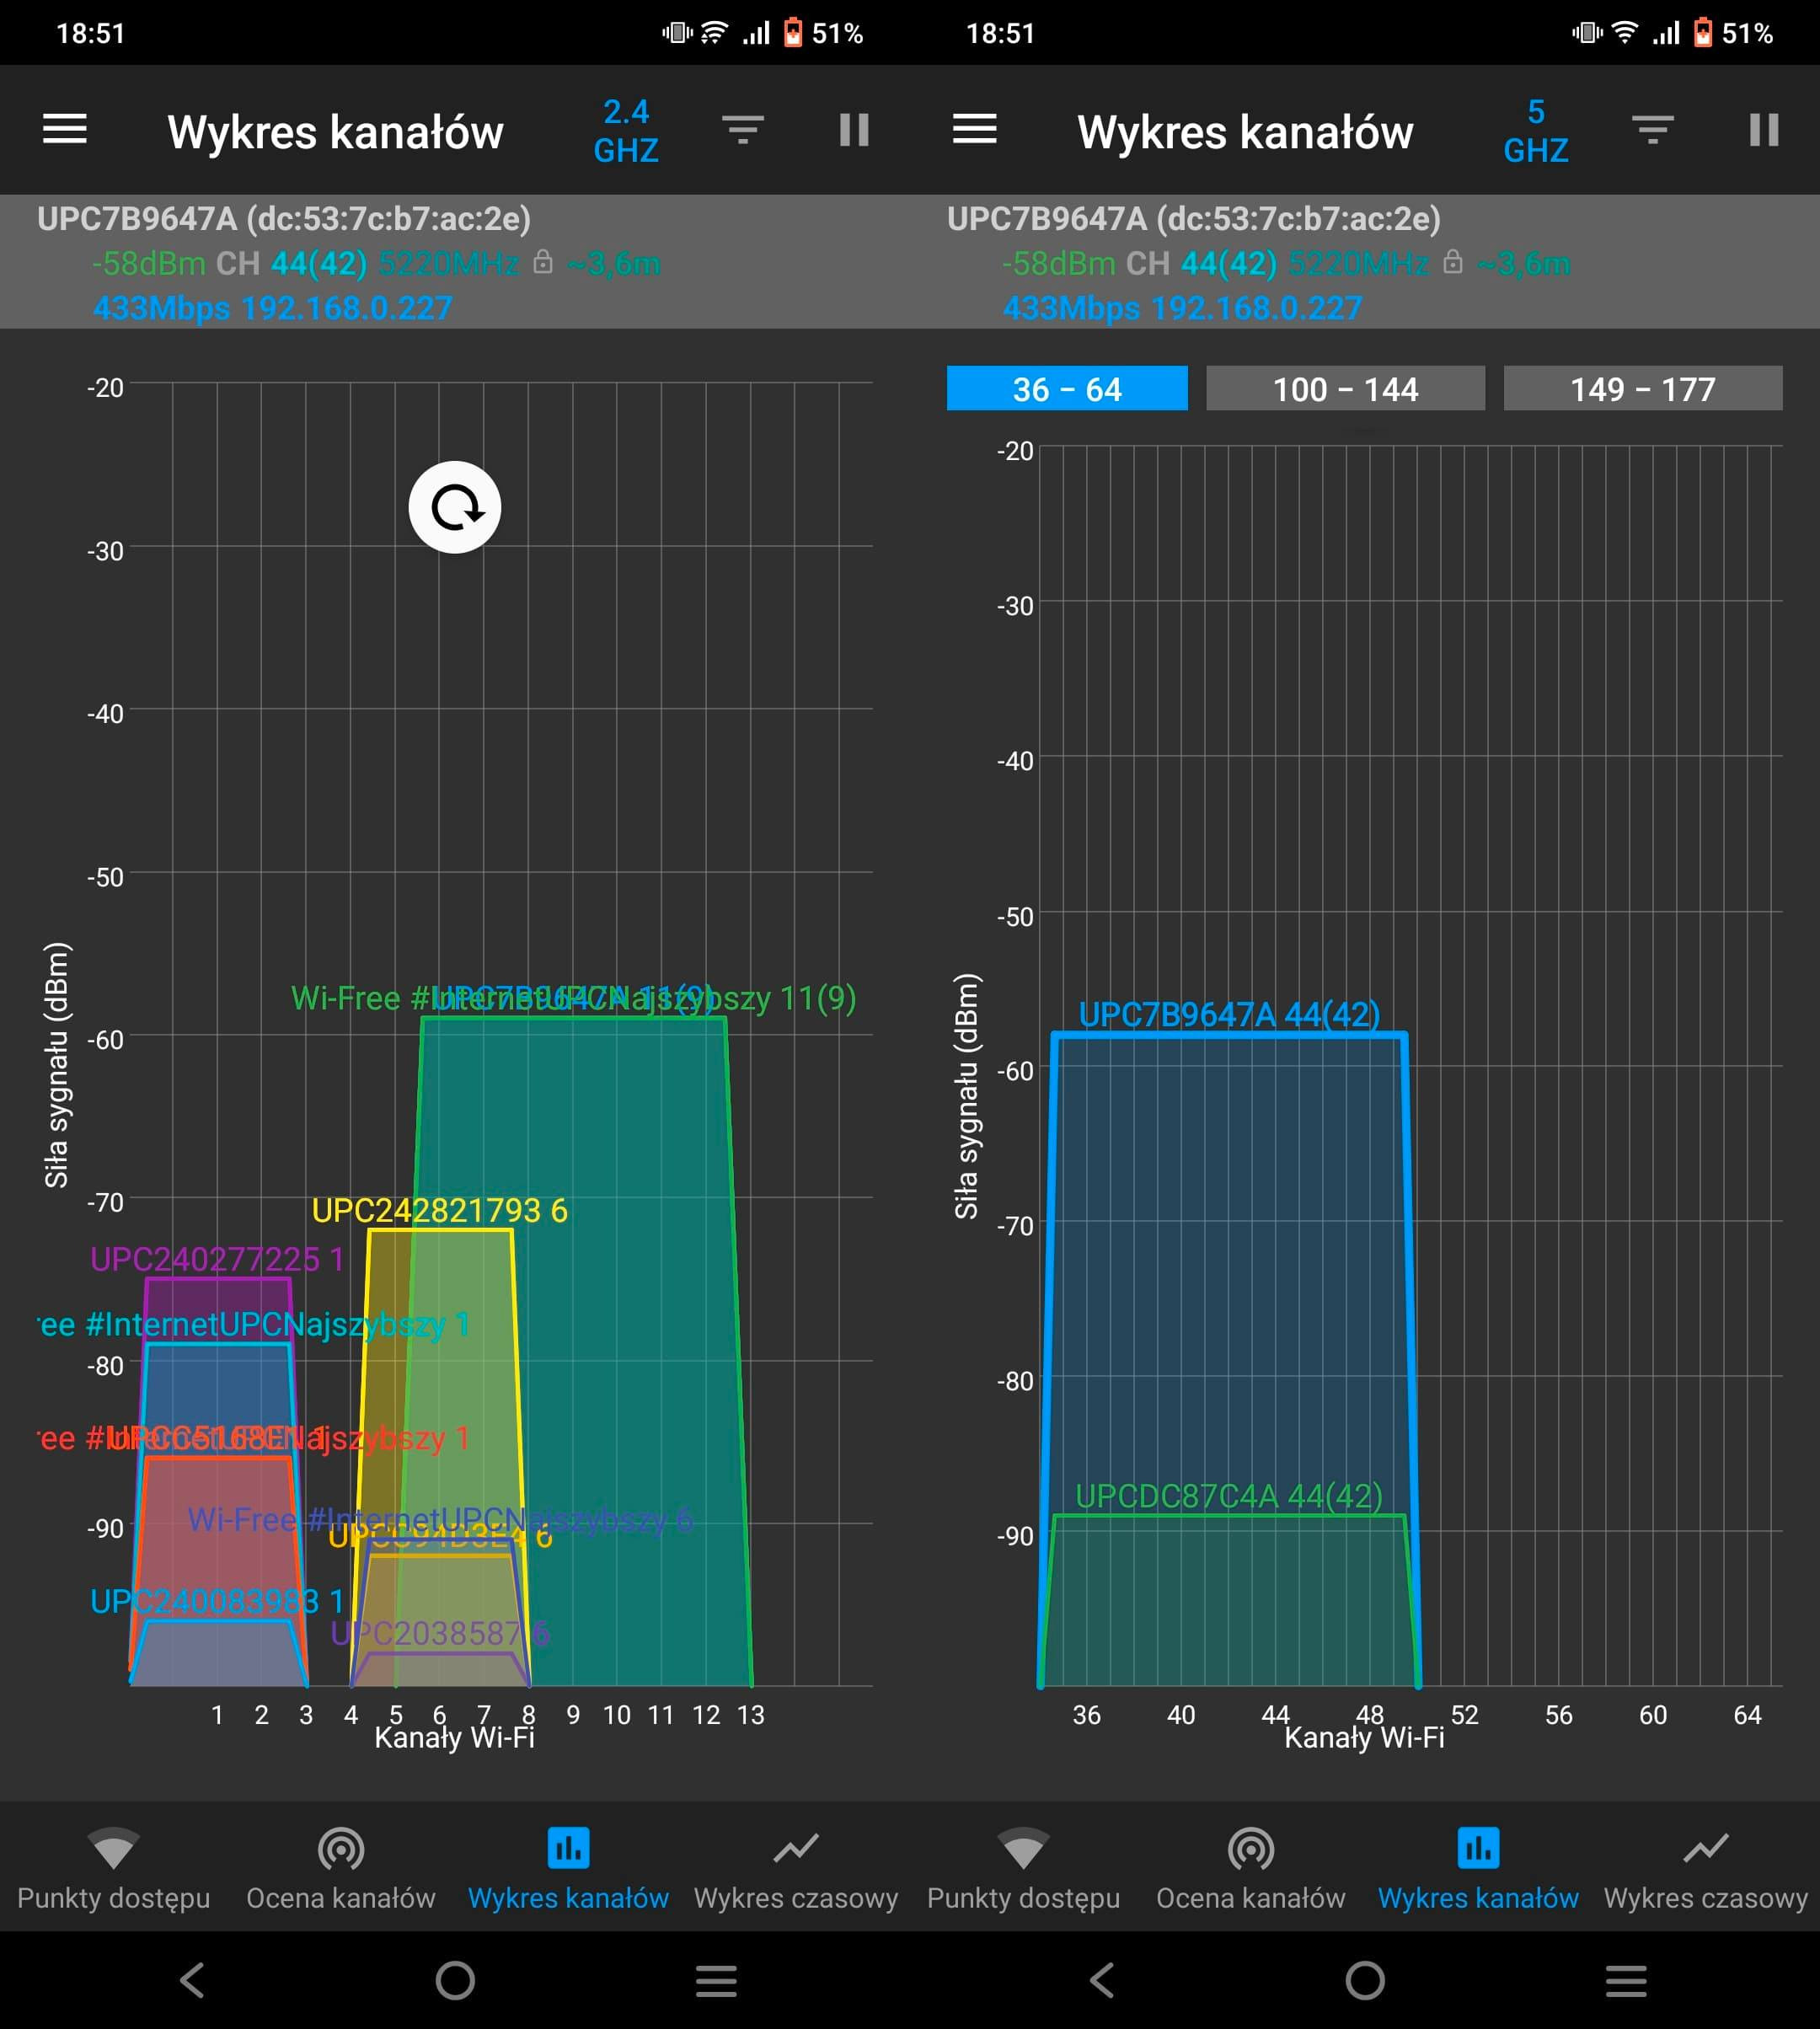
\includegraphics[scale=0.23]{image.jpg}
\end{figure}

\end{document}